% 请用XeLaTeX编译~ 编辑器使用UTF-8模式~
\documentclass[a4paper,10pt]{article}
%Chinese
	\usepackage[fontset=fandol]{ctex}
	\xeCJKsetup{underdot = {
		boxdepth=0pt, format=\huge, depth=.4em
	}}
	\usepackage[datesep=/]{datetime2}
%Presettings
	\usepackage[table]{xcolor}
	\usepackage{graphicx}
	\usepackage[font={sf}]{caption}
	\usepackage[above]{placeins}
%MathSetting
	\let\latexointop\ointop
	\usepackage{amsmath,amssymb,esint,upgreek,textcomp}
	\usepackage[only,sslash]{stmaryrd}
	\usepackage{nicefrac,eqnarray}%amsthm
	\usepackage{bm,mathrsfs,mathtools,physics,siunitx}
	\usepackage{enumitem,stackengine,titling,varwidth}
	\usepackage{tikz}
	\usepackage{resizegather,empheq}
	\usetagform{default}
	\usepackage{calligra}
	\let\ointop\undefined
	\let\ointop\latexointop%oint unchanged by esint
	\DeclareMathAlphabet{\mathcalligra}{T1}{calligra}{m}{n}
	\DeclareFontShape{T1}{calligra}{m}{n}{<->s*[2.2]callig15}{}
	\DeclarePairedDelimiter\ave{\langle}{\rangle}
	\newcommand{\scriptr}{\mathcalligra{r}\,}
	\newcommand{\rvector}{\pmb{\mathcalligra{r}}\,}
	\newcommand{\sinc}{\operatorname{sinc}}
	\newcommand\inlineeqno{\stepcounter{equation}\ (\theequation)}
	\newcommand{\mbb}[1]{\mathbb{#1}}
	\newcommand{\mrm}[1]{\mathrm{#1}}
	\newcommand{\mcal}[1]{\mathcal{#1}}
	\newcommand*\bbox[1]{\fbox{\hspace{1em}\addstackgap[5pt]{#1}\hspace{1em}}}
	\newcommand\scalemath[2]{\scalebox{#1}{\mbox{\ensuremath{\displaystyle #2}}}}
	\newcommand\raisemath[2]{\raisebox{#1\depth}{${#2}$}}
	\empheqset{box=\bbox}
	\allowdisplaybreaks[2]
	\sisetup{separate-uncertainty=true,range-phrase=\,\textasciitilde\,,arc-separator = \,}
%ParagraphSetting
	\setlength{\parskip}{.3\baselineskip}
	\usepackage[defaultlines=2,all]{nowidow}
	\postdisplaypenalty=50
%PageSetting
	\usepackage{array,booktabs,tabularx,tabu}
	\usepackage[colorlinks=true,linkcolor=blue]{hyperref}
	\usepackage[vmargin={4cm,5cm},hmargin=3cm]{geometry}
	\renewcommand{\tableautorefname}{\tablename}
	\renewcommand{\figureautorefname}{\figurename}
	\setlist{itemsep=0pt,topsep=0pt,labelindent=\parindent,leftmargin=0pt,itemindent=*}
	\setlength{\headsep}{2.2cm}
	\setlength{\droptitle}{-2.2cm}
	\usepackage{fancyhdr,lastpage}
	\pagestyle{fancy}
	\fancyhf{}
	\lhead{
		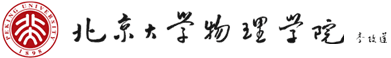
\includegraphics[height=3.2em]{PKUPhy}
		\vspace{-3ex}
		}
	\rhead{
		\itshape\small
		\begin{tabular}{rr}
			\multicolumn{2}{r}{Bryan} \\[.3em]
			学号:   & 1500000000 \\[.2em]
			实验日期:& 2017/03/03 \\[.5em]
		\end{tabular}\hspace{-1em}
		}
	\cfoot{--\ \thepage\,/\,\pageref{LastPage} \ --}
	\renewcommand{\headrulewidth}{0.1pt}
	\renewcommand{\headrule}{
		\vbox to 2pt{
		\hbox to \headwidth{\dotfill}\vss}}
%TitleSettings
	\pretitle{\begin{center}}
	\posttitle{\par\end{center}\vspace{-6mm}}
	\predate{}
	\postdate{\vspace{-4mm}}
%Title
	\title{\textit{\large 实验二十一}\\[2mm]
		\textbf{\LARGE 观察光的偏振现象}}
	\author{\textit{Bryan}}
	\date{}
	
	\newcommand{\tto}{\textrightarrow}

\begin{document}
\maketitle
\thispagestyle{fancy}
\section{基本的偏振现象}
\subsection{Brewster定律之检验}
%	实验现象、理论解释。
	据Brewster定律,当自然光沿Brewster角入射到介质表面上时,其p波反射率为0, 这便得到了只有s分量的线偏反射光。由此定律便可构造偏振光镜,如图所示:
	\begin{figure}[!h]
	\centering
	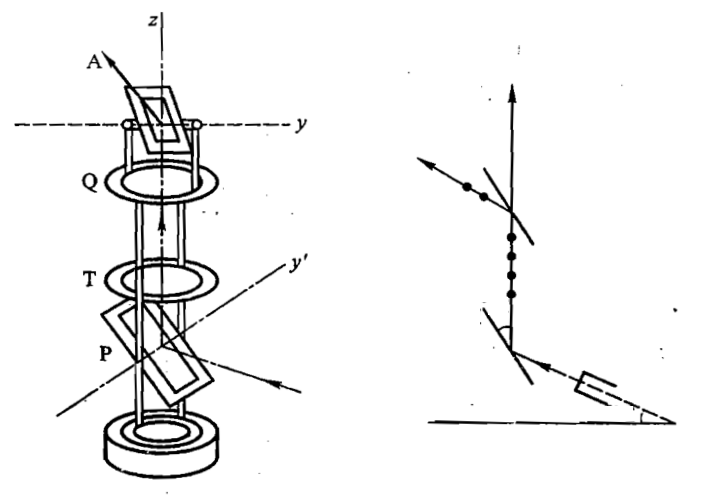
\includegraphics[width=.5\linewidth]{brewster}
	\caption{偏振光镜及其光路示意图}
	\small\itshape 摘自实验教材
	\end{figure}\FloatBarrier\itshape
	装置P的入射角即为Brewster角。此时,用偏振片检验P的反射光,可见检偏器透振方向沿$y'$时透光最大,沿垂直$y'$时几乎消光。由此可得,P的反射光基本可近似为沿$y'$方向即s方向的线偏振光,与Brewster定律吻合。\normalfont
	
	进一步,绕$z$轴转动A,观察到如下现象:
	\begin{enumerate}
	\item 两反射面平行时,A之反射光极强,透射光较弱;转动A, 此时光线入射角不变,然而反射光渐弱,透射光渐强;转角达 \ang{90} 时,反射极弱,透射极强;继续转动A, 光强又逐步增大,至 \ang{180} 时光强与 \ang{0} 情形基本一致。顺、逆时针转动规律一致。
	\item 注意到,透射光强的变化趋势与反射光强变化趋势恰好相反。
	\end{enumerate}
	
	这一现象与Brewster定律一致。绕$z$轴转动A的过程中,入射角恒为Brewster角,然在介质A看来,入射光的p, s成分发生了变化;具体而言,记转角为$\phi$, 有:
	\[ E_s = E_{s,0} \cos\phi,\quad
		E_p = E_{p,0} \sin\phi, \]
	由Brewster定律,此时反射光仅有s波成分,其强度正比于$\abs{E_s}^2$即$\cos^2\phi$, 故有上述的振荡变化规律。结合能量守恒,即可解释透射光的变化规律。
\pagebreak[1]
	
	$\phi = \pm\frac{\pi}{2} = \pm\ang{90}$处是理论上的反射光消光位置,实际反射光存在但极弱;由于激光输入的光强极大,此时的能量反射率微乎其微,可以认为是因仪器精度有限导致的误差,不违背Brewster定律。
	
	在此位置上,进一步绕$y$轴转动A, 此时入射角$i$发生了变化,偏离了Brewster角$i_B$. 观察反射、透射光强,有如下现象:
	\begin{enumerate}[noitemsep]
	\item 入射角$i$偏离$i_B$愈显著,反射光愈强;尤其在掠入射($i\to\ang{90}$)时,反射光达到最强,几乎不可见透射光;
	\item 同样,透射光强的变化趋势与反射光强变化趋势恰好相反。
	\end{enumerate}
	
	这同样与Brewster定律一致。更精细的描述需要用到Fresnel公式;事实上,此时对A来说,入射光全为p波成分,有p波振幅反射率:
	\begin{equation}
		r_p = \frac{n\cos i - \cos r}
			{n\cos i + \cos r}
		= \frac{\tan\pqty{i - r}}
			{\tan\pqty{i + r}}
	\end{equation}
	其中$r$为折射角,$n$为介质相对空气的折射率。结合$n\sin r = \sin i$, 可作出光强反射率$\abs{r_p}^2$对$i$的依赖关系示意图;
	\begin{figure}[!h]
	\centering
	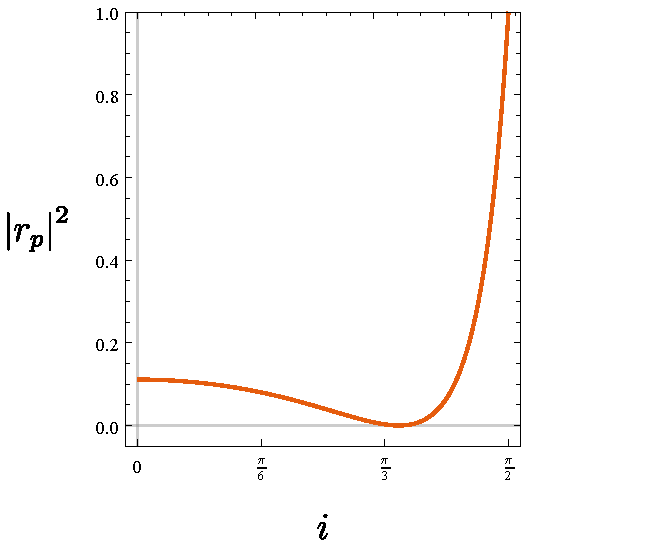
\includegraphics[width=.7\linewidth]{rpgraph}
	\caption{光疏到光密介质的反射率变化规律}
	\small\itshape 取$n=2$计算得到
	\end{figure}
	由图可见,实验现象与理论吻合。
\subsection{晶体的双折射现象}
	当自然光沿非光轴方向入射到单轴晶体上时,晶体内出现两束折射光。其中一束满足Snell折射定律, 此即o光;另一束不满足Snell定律,此即e光。
	\begin{figure}[!h]
	\centering
	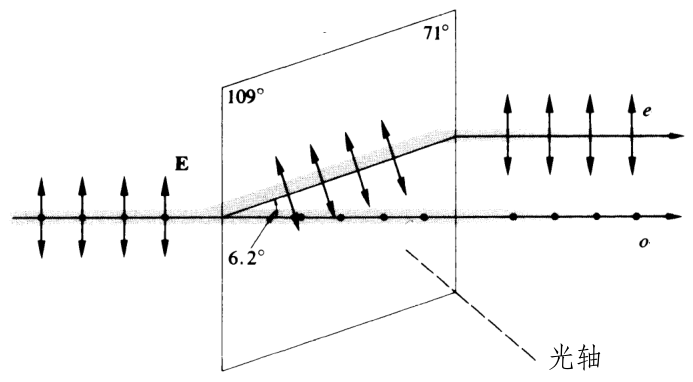
\includegraphics[width=.55\linewidth]{birefringence}
	\caption{方解石的双折射光路示意图}
	\end{figure}\FloatBarrier
	实际观察,可见如下现象:
	\begin{enumerate}
	\item 透过方解石截面看下方光点,可见两像;转动晶体,其中一个不动,另一绕之转动;
	\item 加上偏振片观察,相对晶体转动偏振片,两光点的亮暗均会变化,变化规律相反;在一定角度上只能看见其中一个光点,此时旋转偏振片,原可见光点亮度逐渐减弱,原不可见光点亮度逐渐增大;至 \ang{90} 处原不可见光点达到最亮,原可见光点消失不见。
	\item 透过方解石的磨面观察,则只可见一个光点,不随晶体转动而变动;
	\end{enumerate}
	
	由实验现象总结可知,方解石中的两束光分开传播,且均为线偏光,偏振方向正交;寻常光(o光)不随晶体转动而变化,非寻常光(e光)的传播方向则跟随晶体发生转动。这与图示所描述的光路一致。
	
	透过磨面观察时,光线沿光轴传播,从而没有双折射现象。
\section{波晶片对偏振光的影响}
\subsection{\texorpdfstring{$\lambda/2$}{λ/2}波晶片
	变换线偏光的偏振方向}
	利用起偏、检偏器P、A构成如下光路,在其中加入波晶片C观察透射光现象。取C为$\lambda/2$波晶片,记录现象如下:
	\begin{enumerate}
	\item 首先不加入C, 旋转A, 记转角为$\theta$, 可见光强按照$\cos^2\theta$规律变化,转一圈出现两次消光,这是典型的线偏光特征,与Malus定律一致。
	\item 将P转至刻度为$\theta = \ang{0}$处,\textit{\CJKunderdot{定义}}此时P的透振方向为竖直方向;转A达到消光,此时粗测A的刻度$\theta'_0 \approx \ang{23}$. 加入$\lambda/2$片,将之转动一圈,出现4次消光。
	\item 固定$\lambda/2$片而转动A, 则只见2次消光。
	\end{enumerate}
	
	\begin{figure}[!h]
	\centering
	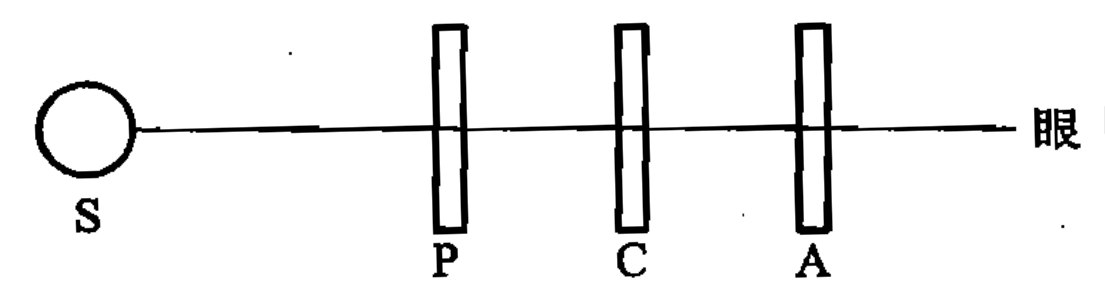
\includegraphics[width=.5\linewidth]{waveplate}
	\caption{观察波晶片透射光的偏振情况}
	\end{figure}
	
	可见,透过$\lambda/2$片的光线依然是线偏振的,但是其入射、出射光偏振方向发生了变化。记$\lambda/2$片转角为$\alpha$, $\lambda/2$片在入射光的o, e分量中引入了$\pi$的相差,从而导致偏振方向由相对光轴的$-\alpha$变为$+\alpha$, 转过了$2\alpha$角度。透过检偏器的光强按:
	\[ I \propto \sin^2 2\alpha \]
	规律变化,因此出现4次消光,与实验现象吻合。
	
	进一步定量检验上述规律。将$\lambda/2$转到消光位置固定,转动P改变$\theta$, 在反方向转动A使消光,记录A转过的角度(负数):
	\[ \Delta\theta' \equiv \theta' - \theta'_0,\ 
		\mod \ang{360} \]
	有如下结果:
	\begin{table}[!h]
	\centering
	\caption{$\lambda/2$旋转线偏光之角度测定数据表}
	\begin{tabular}{c|@{\hspace{1.5em}}SSSSSSS@{\hspace{-.5em}}}
	\toprule
		$\theta/\si{\degree}$ &
		0     & 15    & 30    & 45    & 60    & 75    & 90  \\
		$\theta'/\si{\degree}$ &
		23    & 8     & 352   & 338   & 322   & 308   & 292 \\
		$\Delta\theta'/\si{\degree}$ &
		0     & -15   & -31   & -45   & -61   & -75   & -91 \\
	\bottomrule
	\end{tabular}
	\end{table}
	
	\noindent 可见,在误差允许的范围内,$\theta \approxeq - \Delta\theta'$, 这与上述理论分析吻合。
\subsubsection{应用:显色偏振实验}
	用白光源照射置于正交偏振片之间的各向异性胶纸,可见显色偏振现象。实验如下:
	\begin{enumerate}
	\item 转动置于正交偏振片之间的胶纸使消光,在此位置上继续将样品旋转 \ang{45}, 此时样品上由厚至薄依次出现\textit{紫——绿——黄——橙}的颜色;
	\item 逐步旋转检偏器,样品显现的颜色发生渐变;当起偏、检偏器透振方向一致(即转过 \ang{90})时,样品颜色变为\textit{黄——红——紫——蓝},恰为前面颜色之补色。
	\end{enumerate}
	
	事实上,对旋转 \ang{45} 后的样品来说,入射光偏振方向与o, e方向之夹角均为 \ang{45}. 此时,若该层胶纸对波长$\sim\lambda$的光来说恰是$\lambda/2$波晶片,则出射光也是线偏光,偏振方向相对入射光转过$2\times\ang{45} = \ang{90}$, 恰能完全通过检偏器。
	
	胶纸显示出$\sim\lambda$的颜色,说明在透过检偏器的光当中,波长在$\lambda$附近的光占主要成分,即意味着该段胶纸可视为对应的$\lambda/2$波晶片。考虑相邻段胶纸的颜色差异,应有:
	\[ \frac{\Delta\lambda}{2}
		\equiv \Delta L = d\,\Delta n \]
	由此可估计胶纸厚度。然而,此处对$\Delta n$没有概念,因此未做具体计算。
\subsection{\texorpdfstring{$\lambda/4$}{λ/4}波晶片
	使线偏光变化为椭偏光}
	重复与上述$\lambda/2$波晶片类似的实验,只是将光路图中的C替换为$\lambda/4$波晶片,有如下现象:
	\begin{table}[!h]
	\centering
	\caption{$\lambda/2$旋转线偏光之角度测定数据表}
	\begin{tabu} to .8\linewidth {X[c,1]X[l,3]X[c,2]}
	\toprule
		$\theta/\si{\degree}$ &
		\textbf{A转一圈可见现象} & \textbf{C出射光偏振态} \\
	\midrule
		0     & 消光\tto 亮\tto 消光\tto 亮    & 线偏 \\
		15    & 暗\tto 亮\tto 暗\tto 亮,无消光 & 椭偏 \\
		30    & 同上,光强变化不那么显著         & 椭偏 \\
		45    & 光强基本恒定                   & 圆偏 \\
		60    & 亮\tto 暗\tto 亮\tto 暗,无消光 & 椭偏 \\
		75    & 同上,光强变化更加显著           & 椭偏 \\
		90    & 亮\tto 消光\tto 亮\tto 消光    & 线偏 \\
	\bottomrule
	\end{tabu}
	\end{table}\FloatBarrier
	\noindent 可见,出射光是椭圆偏振光,这是由$\lambda/4$波晶片在o, e分量之间引入$\frac{\pi}{2}$相差所导致的。当入射光恰好沿光轴时,得到线偏光;当入射光与波晶片o, e轴均夹 \ang{45} 时,得到圆偏光。
\subsubsection{应用:椭偏光与部分偏振光的产生及检验}
	上述实验可以产生椭圆偏振光。如果只通过检偏器A观察,椭偏光与\textit{部分偏振光}有完全类似的特性;其中,部分偏振光是令光线按Brewster角入射玻璃片堆、收集透射光得到的。
	
	\itshape 由于入射光的s分量在玻璃片堆中一次次反射,几乎消耗殆尽,得到的是仅含有少量s成分却含有大量p成分的透射光,此即部分偏振光。\normalfont
	
	可通过以下光路区分椭偏光与部分偏振光。
	\begin{figure}[!h]
	\centering
	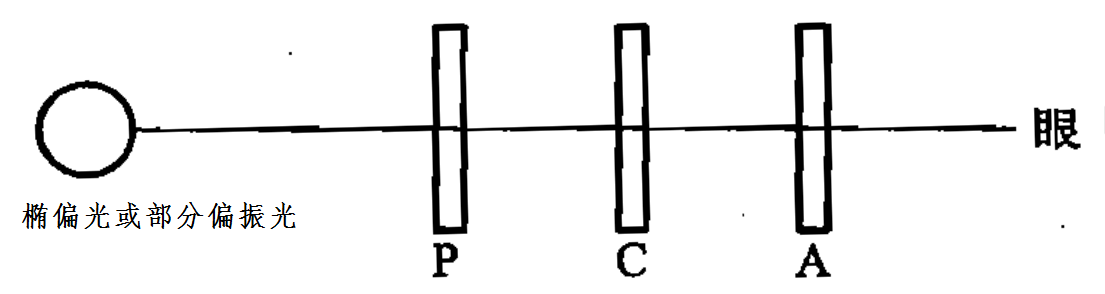
\includegraphics[width=.7\linewidth]{identify}
	\caption{检验椭偏光与部分偏振光}
	\end{figure}\FloatBarrier
	
	假定入射光为椭偏光,考虑如下步骤:
	\begin{enumerate}
	\item 使光入射偏振片P, 调整偏振片的方向使透过P的光强最小,此时该偏振片的透振方向与椭圆的短轴平行;
	\item 不加入C, 只在P后再加一偏振片A使消光;此时A的透振方向沿椭圆长轴;
	\item 在两偏振片间加入$\lambda/4$片C, 调整使消光。此时,波晶片的o, e方向分别对应两偏振片的透振方向,进而对应椭圆的长短轴;也就是说,若以o, e方向为坐标轴,该椭偏光光矢量的变化轨迹为正椭圆;
	\item 移走P, 让椭偏光直接通过C, 应当得到线偏光。此时调整E, 可以完全消光。
	\end{enumerate}
	对部分偏振光重复上述步骤,则并不能完全消光(\textit{部分偏振光通过$\lambda/4$片并不能得到线偏光}),由此便将椭偏光与部分偏振光区分开了。
	
	\vfill\noindent\itshape\footnotesize
	\hfill Last edited: \today\ \copyright\ Bryan
\end{document}
% Copyright © Bryan